\begin{frame}[allowframebreaks]{Where are we heading?}
\begin{columns}
    \begin{column}{0.7\textwidth}
       \begin{figure}
            \centering
            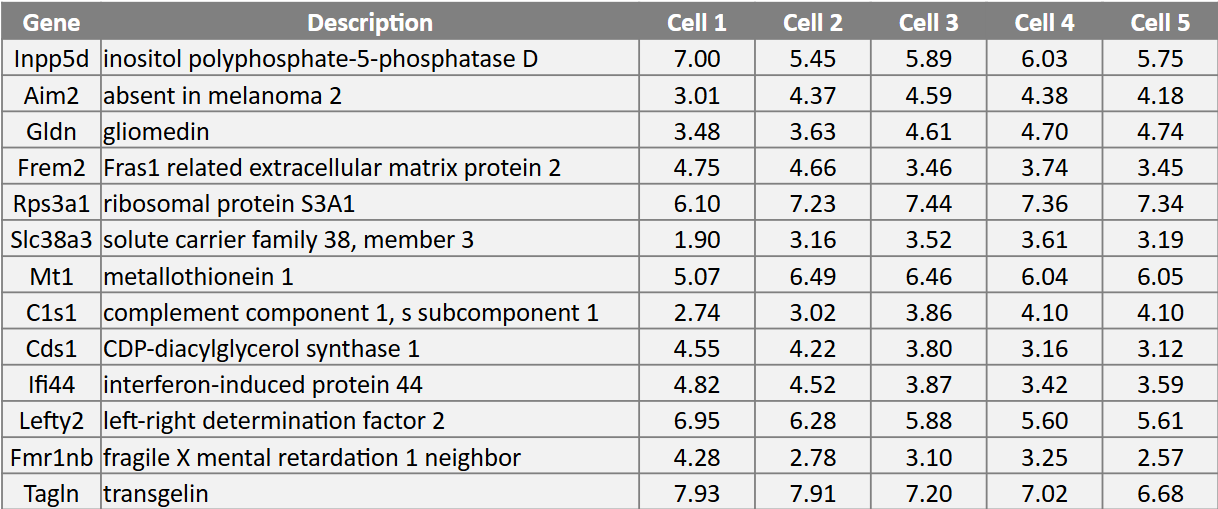
\includegraphics[width=1.05\textwidth,keepaspectratio]{images/dul/gene-datapoints.png}
            \caption{Original Points}
        \end{figure}
        \vspace{1em}
        \begin{itemize}
            \item Each dot is a cell.
            \item Groups of dots are similar cells.
            \item Separation of groups could be interesting biology.
        \end{itemize}
    \end{column}
    \begin{column}{0.3\textwidth}
        \begin{figure}
            \centering
            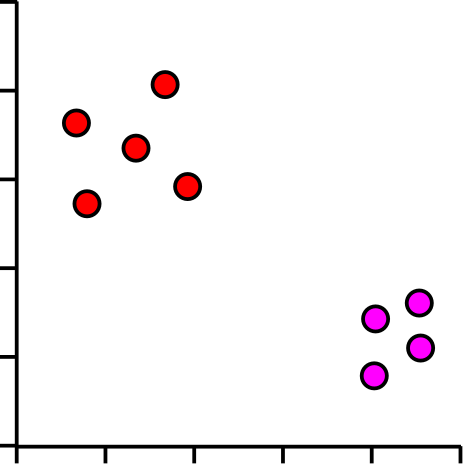
\includegraphics[width=1\textwidth,keepaspectratio]{images/dul/gene-datapoints-plot.png}
            \caption{Clusters identified by DBSCAN}
        \end{figure}
    \end{column}
\end{columns}
\end{frame}


\begin{frame}[allowframebreaks]{Too much data!}
    \begin{itemize}
        \item 5000 cells and 2500 measured genes
        \item Realistically only 2 dimensions we can plot (x, y)
    \end{itemize}
\begin{columns}
    \begin{column}{0.33\textwidth}
       \begin{figure}
            \centering
            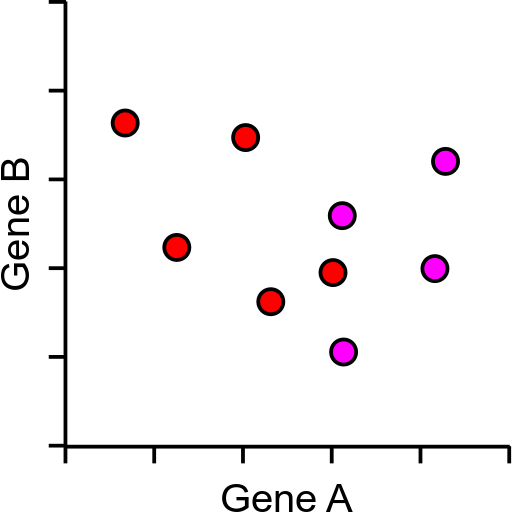
\includegraphics[width=1\textwidth,keepaspectratio]{images/dul/gene-AB.png}
        \end{figure}
    \end{column}
    \begin{column}{0.33\textwidth}
        \begin{figure}
            \centering
            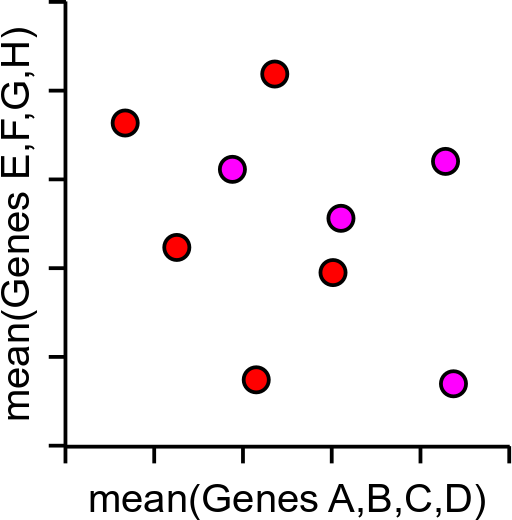
\includegraphics[width=1\textwidth,keepaspectratio]{images/dul/genes-mean.png}
        \end{figure}
    \end{column}
    \begin{column}{0.33\textwidth}
        \begin{figure}
            \centering
            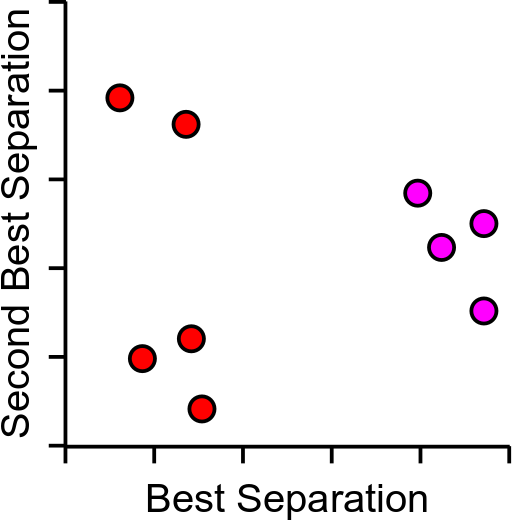
\includegraphics[width=1\textwidth,keepaspectratio]{images/dul/genes-separations.png}
        \end{figure}
    \end{column}
\end{columns}
\end{frame}

\begin{frame}[allowframebreaks]{Principal Component Analysis (PCA)}
    \begin{itemize}
        \item Principal Component Analysis (PCA) is a method for optimally summarizing large, multi-dimensional datasets.
        \item PCA identifies a smaller number of dimensions (ideally 2) that retain most of the useful information present in the original data.
        \item The technique constructs a set of new variables, called Principal Components (PCs), which are linear combinations of the original variables.
        \item Each Principal Component represents a specific weighted sum of the original features. For example:
        \begin{equation*}
            \text{PC} = (10 \times \text{GeneA}) + (3 \times \text{GeneB}) + (-4 \times \text{GeneC}) + (-20 \times \text{GeneD}) + \ldots
        \end{equation*}
        \item By projecting the data onto these principal components, PCA reduces dimensionality while preserving as much variance (information) as possible.
    \end{itemize}

    \framebreak

    \begin{itemize}
        \item Principal Component Analysis (PCA) is a method for optimally summarizing large, multi-dimensional datasets.
        \item PCA identifies a smaller number of dimensions (ideally 2) that retain most of the useful information present in the original data.
        \item The technique constructs a set of new variables, called Principal Components (PCs), which are linear combinations of the original variables.
        \item Each Principal Component represents a specific weighted sum of the original features. For example:
        \begin{equation*}
            \textcolor{gray}{\text{PC}} = \textcolor{gray}{(}10 \textcolor{gray}{\times \text{GeneA}) + (}3 \textcolor{gray}{\times \text{GeneB}) + (}-4 \textcolor{gray}{\times \text{GeneC}) + (}-20 \textcolor{gray}{\times \text{GeneD}) + \ldots}
        \end{equation*}
        \item By projecting the data onto these principal components, PCA reduces dimensionality while preserving as much variance (information) as possible.
    \end{itemize}

    Simple example using 2 genes and 10 cells

\end{frame}

\begin{frame}[allowframebreaks]{How does PCA work?}    
    Simple example using 2 genes and 10 cells
    \vspace{1cm}
    \begin{columns}
    \begin{column}{0.5\textwidth}
        \begin{figure}
            \centering
            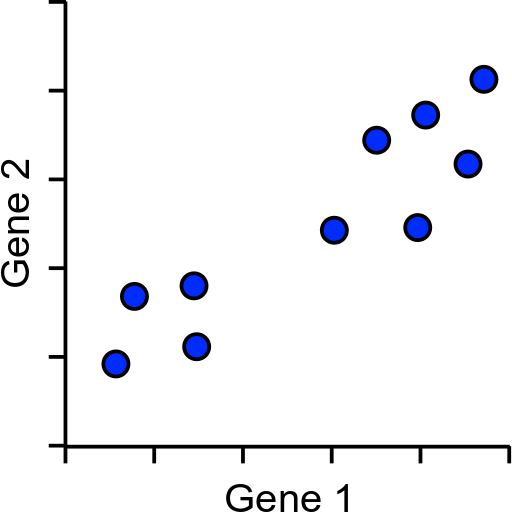
\includegraphics[width=1\textwidth,keepaspectratio]{images/dul/dim-reduce/points.png}
        \end{figure}
    \end{column}
    \begin{column}{0.5\textwidth}
        \begin{figure}
            \centering
            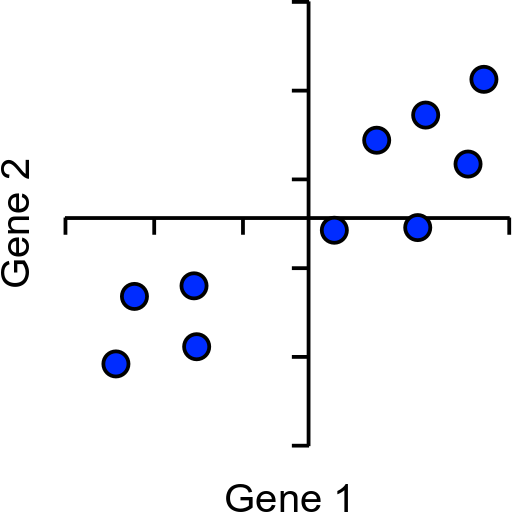
\includegraphics[width=1\textwidth,keepaspectratio]{images/dul/dim-reduce/points-separation.png}
        \end{figure}
    \end{column}
    \end{columns}

    \framebreak

    Find line of best fit, passing through the origin
    \vspace{1cm}
    \begin{columns}
    \begin{column}{0.33\textwidth}
        \begin{figure}
            \centering
            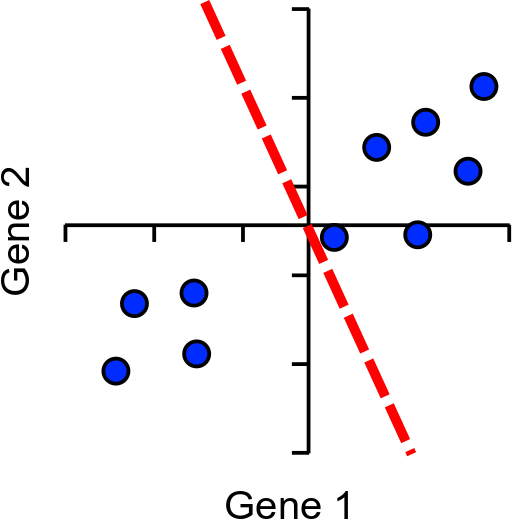
\includegraphics[width=1\textwidth,keepaspectratio]{images/dul/dim-reduce/line-fit.png}
        \end{figure}
    \end{column}
    \begin{column}{0.33\textwidth}
        \begin{figure}
            \centering
            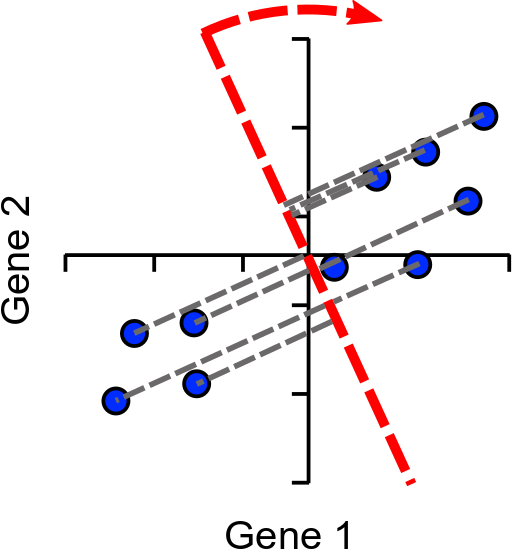
\includegraphics[width=1\textwidth,keepaspectratio]{images/dul/dim-reduce/line-fit-rotate.png}
        \end{figure}
    \end{column}
    \begin{column}{0.33\textwidth}
        \begin{figure}
            \centering
            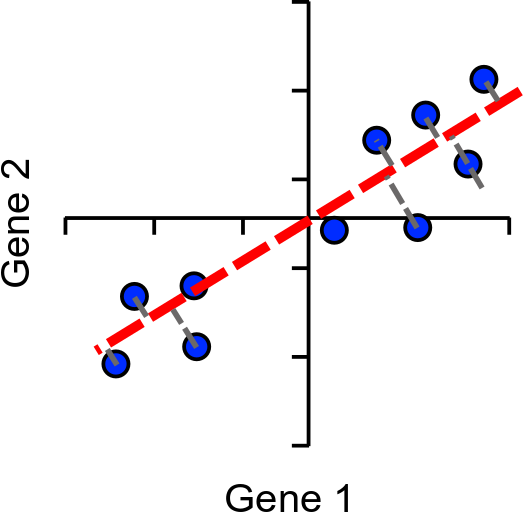
\includegraphics[width=1\textwidth,keepaspectratio]{images/dul/dim-reduce/line-fit-best.png}
        \end{figure}
    \end{column}
    \end{columns}
\end{frame}

\begin{frame}[allowframebreaks]{Assigning Loadings to Genes}    
    \begin{columns}
    \begin{column}{0.5\textwidth}
        \begin{figure}
            \centering
            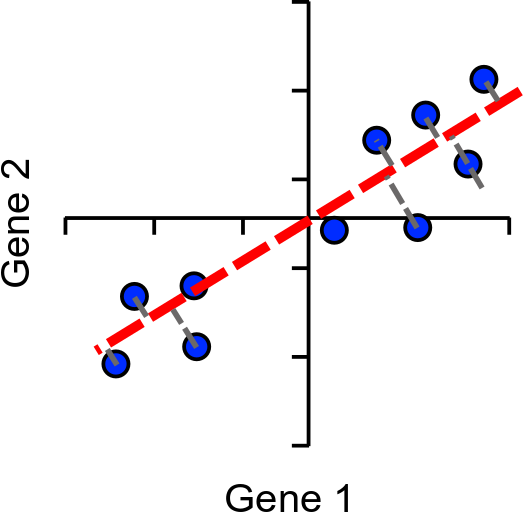
\includegraphics[width=0.8\textwidth,keepaspectratio]{images/dul/dim-reduce/line-fit-best.png}
        \end{figure}
    \end{column}
    \begin{column}{0.5\textwidth}
        \begin{figure}
            \centering
            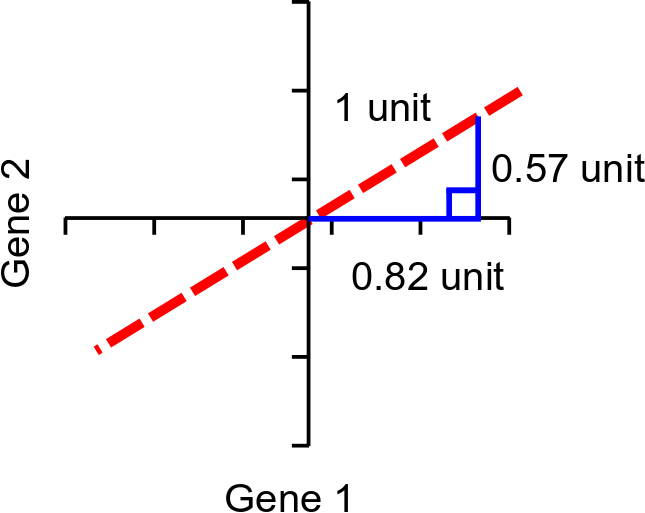
\includegraphics[width=0.8\textwidth,keepaspectratio]{images/dul/dim-reduce/line-eigenvector.png}
            \caption{\textbf{Eigenvector} or Single Vector}
        \end{figure}
    \end{column}
    \end{columns}
    \begin{itemize}
        \setlength{\itemsep}{-0.5em}
        \item \textbf{Loadings} represent the contribution of each gene to the principal component.
        \item For this example using 2 genes and 10 cells:
        \begin{itemize}
            \setlength{\itemsep}{-0.5em}
            \item Gene1 loading: $0.82$
            \item Gene2 loading: $0.57$
        \end{itemize}
        \item A higher loading means the gene has a greater influence on the principal component.
    \end{itemize}
\end{frame}


\begin{frame}[allowframebreaks]{More Dimensions}    
    \begin{columns}
    \begin{column}{0.4\textwidth}
        \begin{figure}
            \centering
            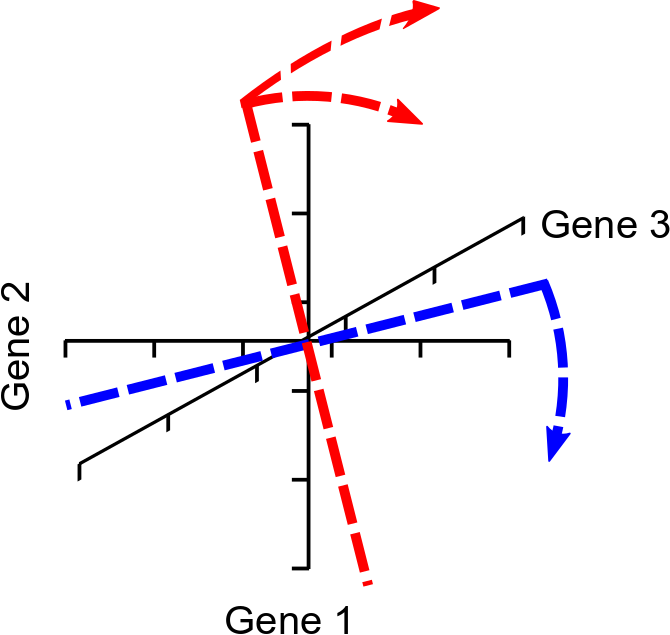
\includegraphics[width=1\textwidth,keepaspectratio]{images/dul/dim-reduce/multi-pcs.png}
        \end{figure}
    \end{column}
    \begin{column}{0.6\textwidth}
        \begin{itemize}
            \item The same idea extends to datasets with more dimensions ($n$ genes).
            \item The first principal component (PC1) finds the direction of maximum variance, rotating in $(n-1)$ dimensions.
            \item The next principal component (PC2) is perpendicular to PC1 and rotates in the remaining $(n-2)$ dimensions.
            \item Each subsequent principal component is always perpendicular to the previous ones, capturing the next largest variance.
            \item The last principal component is the only remaining perpendicular direction.
            \item The number of principal components always equals the number of original genes (features).
        \end{itemize}
    \end{column}
    \end{columns}
\end{frame}


\begin{frame}[allowframebreaks]{Explaining Variance}    
    \begin{itemize}
        \item Each principal component (PC) explains a certain proportion of the total variance in the data. Together, all PCs account for 100\% of the variance.
        \item PC1 always explains the largest amount of variance.
        \item PC2 explains the next largest amount, and so on for subsequent PCs.
        \item Since we typically plot only 2 dimensions (PC1 and PC2), it's important to check how much of the total variance these two PCs explain.
        \item \textbf{How do we calculate this?}
        % \begin{itemize}
        %     \item For each PC, divide the variance explained by that PC by the total variance (sum of variances of all PCs).
        %     \item This gives the proportion (or percentage) of variance explained by each PC.
        %     \item Often visualized using a \textit{scree plot} or by reporting the cumulative variance explained.
        % \end{itemize}
    \end{itemize}

    \framebreak

    \begin{columns}
    \begin{column}{0.5\textwidth}
        \begin{figure}
            \centering
            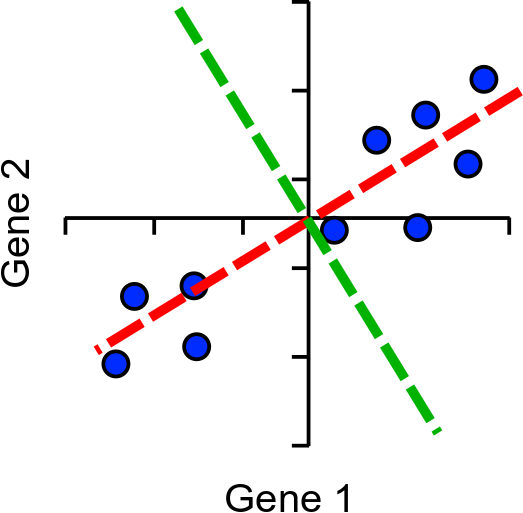
\includegraphics[width=1\textwidth,keepaspectratio]{images/dul/dim-reduce/variance-explained.png}
        \end{figure}
    \end{column}
    \begin{column}{0.5\textwidth}
        \begin{itemize}
            \item Project each data point onto the principal component (PC).
            \item Calculate the distance of each projected point to the origin.
            \item Compute the sum of squared differences (SSD) from the origin.
            \item This SSD is a measure of variance, called the \textit{eigenvalue}.
            \item Divide the SSD by $(\text{number of points} - 1)$ to obtain the actual variance explained by the PC.
        \end{itemize}
    \end{column}
    \end{columns}

    \framebreak

    \begin{columns}
    \begin{column}{0.5\textwidth}
        \begin{figure}
            \centering
            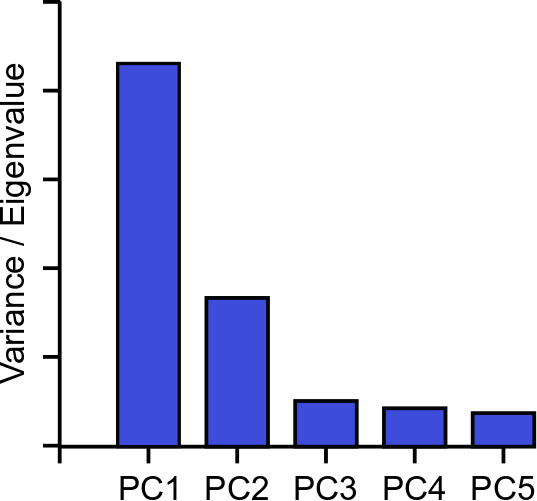
\includegraphics[width=1\textwidth,keepaspectratio]{images/dul/dim-reduce/variance-graph-1.png}
        \end{figure}
    \end{column}
    \begin{column}{0.5\textwidth}
        \begin{figure}
            \centering
            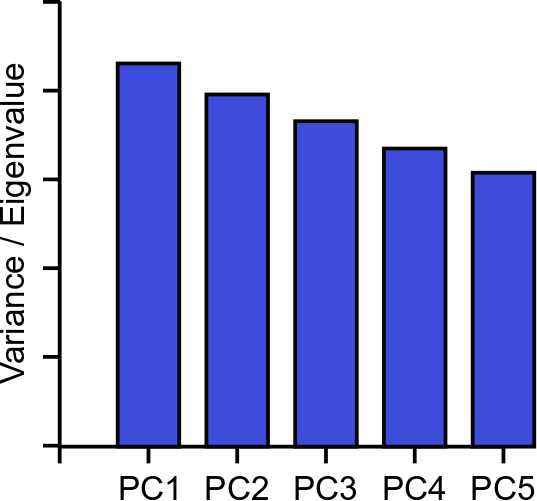
\includegraphics[width=1\textwidth,keepaspectratio]{images/dul/dim-reduce/variance-graph-2.png}
        \end{figure}
    \end{column}
    \end{columns}
\end{frame}


\begin{frame}[allowframebreaks]{So PCA is great then?}
    Kind of\dots
    \begin{columns}
    \begin{column}{0.5\textwidth}
        \begin{figure}
            \centering
            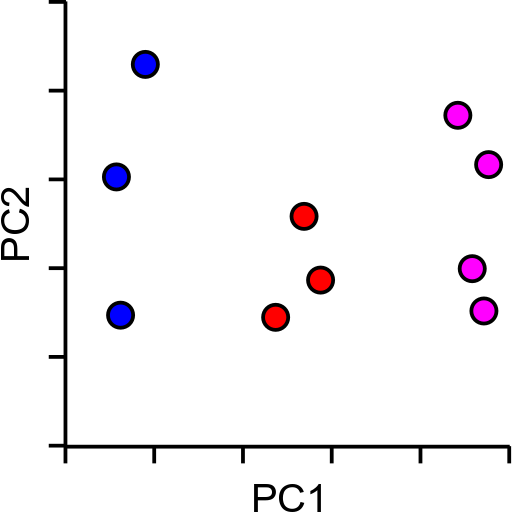
\includegraphics[width=1\textwidth,keepaspectratio]{images/dul/dim-reduce/pca-nonlinear-separation-1.png}
        \end{figure}
    \end{column}
    \begin{column}{0.5\textwidth}
        \begin{figure}
            \centering
            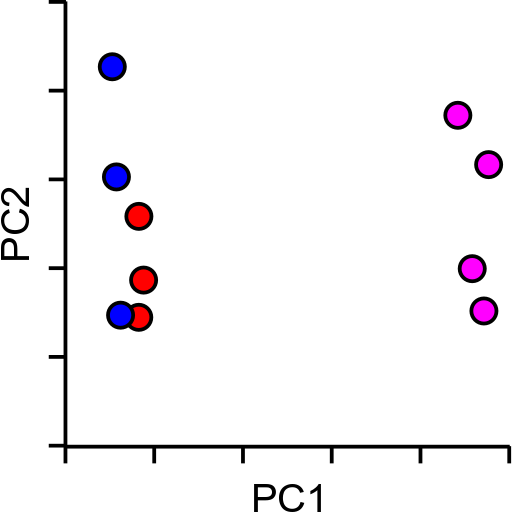
\includegraphics[width=1\textwidth,keepaspectratio]{images/dul/dim-reduce/pca-nonlinear-separation-2.png}
        \end{figure}
    \end{column}
    \end{columns}
    \begin{center}
        Non-linear separation of values
    \end{center}

    \framebreak

    Kind of\dots
    \begin{columns}
    \begin{column}{0.5\textwidth}
        \begin{figure}
            \centering
            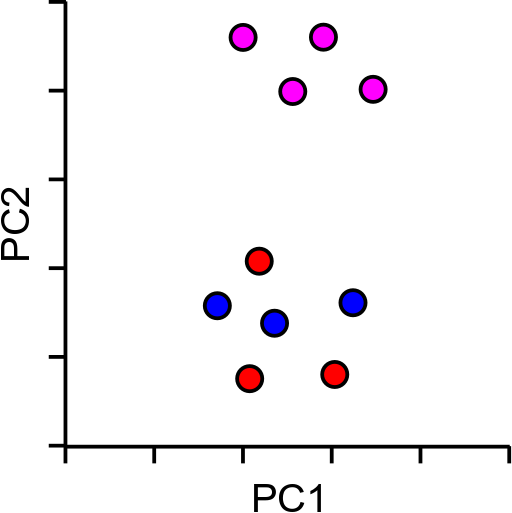
\includegraphics[width=1\textwidth,keepaspectratio]{images/dul/dim-reduce/pca-nonlinear-optimised-1.png}
        \end{figure}
    \end{column}
    \begin{column}{0.5\textwidth}
        \begin{figure}
            \centering
            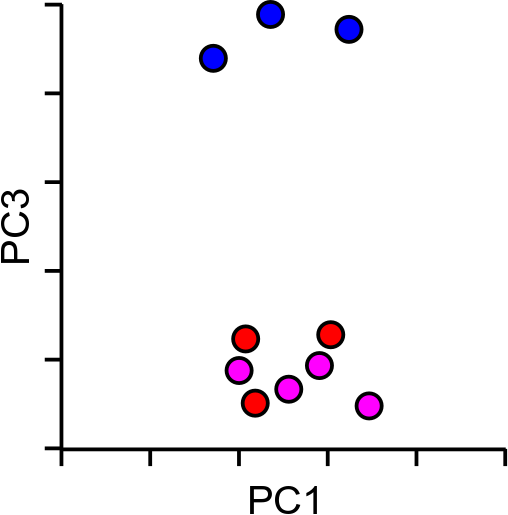
\includegraphics[width=1\textwidth,keepaspectratio]{images/dul/dim-reduce/pca-nonlinear-optimised-2.png}
        \end{figure}
    \end{column}
    \end{columns}
    \begin{center}
        Not optimised for 2-dimensions
    \end{center}
\end{frame}
\begin{frame}[allowframebreaks]{tSNE to the rescue\dots}
    \begin{itemize}
        \item T-Distributed Stochastic Neighbour Embedding
        \item Aims to solve the problems of PCA
        \item Non-linear scaling to represent changes at different levels
        \item Optimal separation in 2-dimensions
    \end{itemize}
\end{frame}

\begin{frame}[allowframebreaks]{tSNE: How does it work?}
    \begin{itemize}
        \item Based around all-vs-all table of pairwise cell to cell distances
        \item Each cell is represented as a point in a high-dimensional space
        \item The pairwise distances are converted into probabilities
    \end{itemize}
    \vspace{1em}
    \begin{columns}
        \begin{column}{0.33\textwidth}
            \begin{figure}
                \centering
                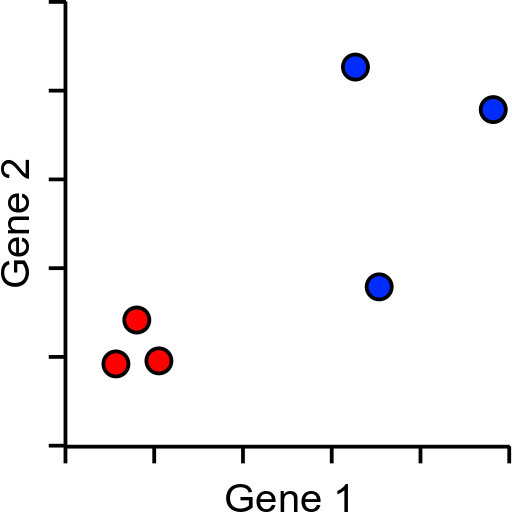
\includegraphics[width=1\textwidth,keepaspectratio]{images/dul/dim-reduce/tsne-points.png}
            \end{figure}
        \end{column}
        \begin{column}{0.33\textwidth}
            \begin{figure}
                \centering
                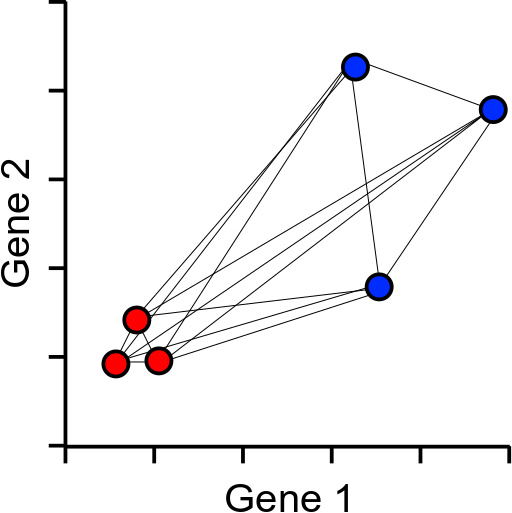
\includegraphics[width=1\textwidth,keepaspectratio]{images/dul/dim-reduce/tsne-graph.png}
            \end{figure}
        \end{column}
        \begin{column}{0.33\textwidth}
            \begin{figure}
                \centering
                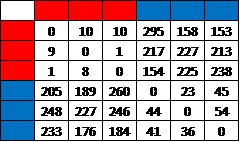
\includegraphics[width=1\textwidth,keepaspectratio]{images/dul/dim-reduce/tsne-matrix.png}
            \end{figure}
        \end{column}
    \end{columns}
\end{frame}

\begin{frame}[allowframebreaks]{tSNE: Underlying idea}
    \begin{figure}
        \centering
        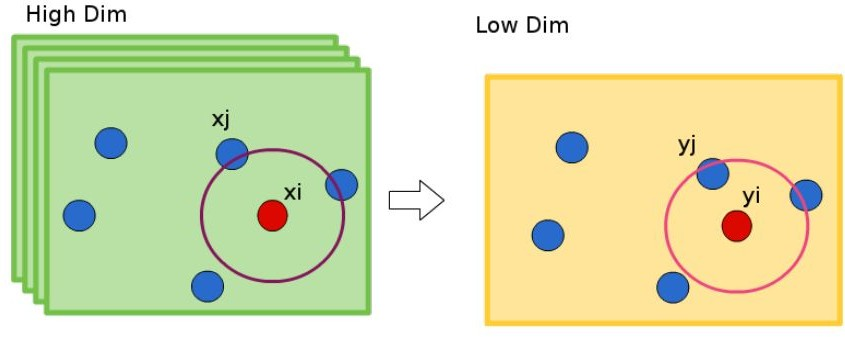
\includegraphics[width=1\textwidth,keepaspectratio]{images/dul/dim-reduce/tsne-high2low.jpg}
    \end{figure}
\end{frame}

\begin{frame}[allowframebreaks]{tSNE: Stochastic Neighbor Embedding}
    \begin{figure}
        \centering
        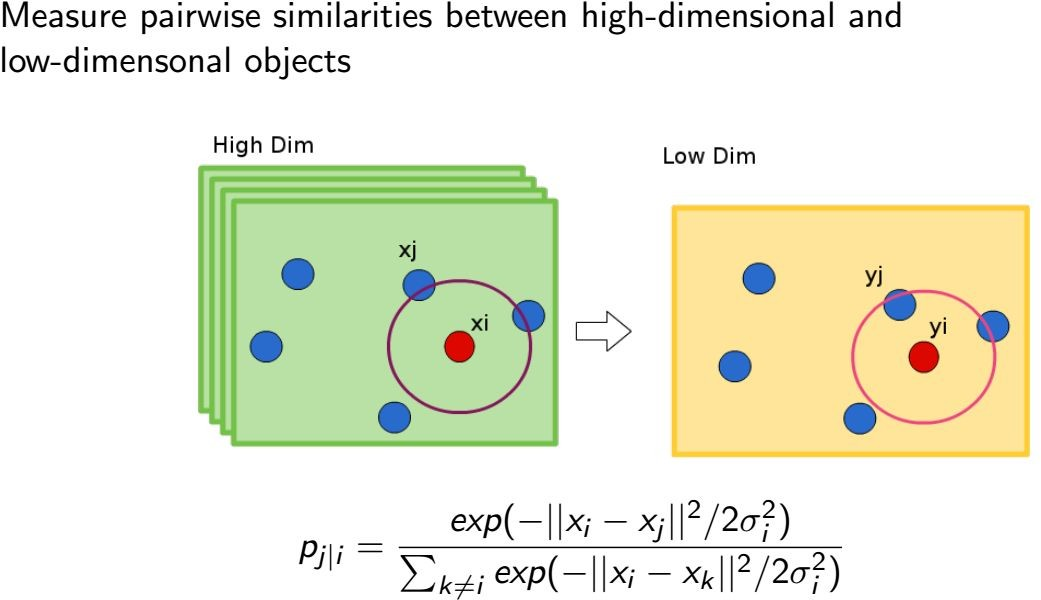
\includegraphics[width=1\textwidth,keepaspectratio]{images/dul/dim-reduce/tsne-stochastic.jpg}
    \end{figure}

    \framebreak

    \begin{figure}
        \centering
        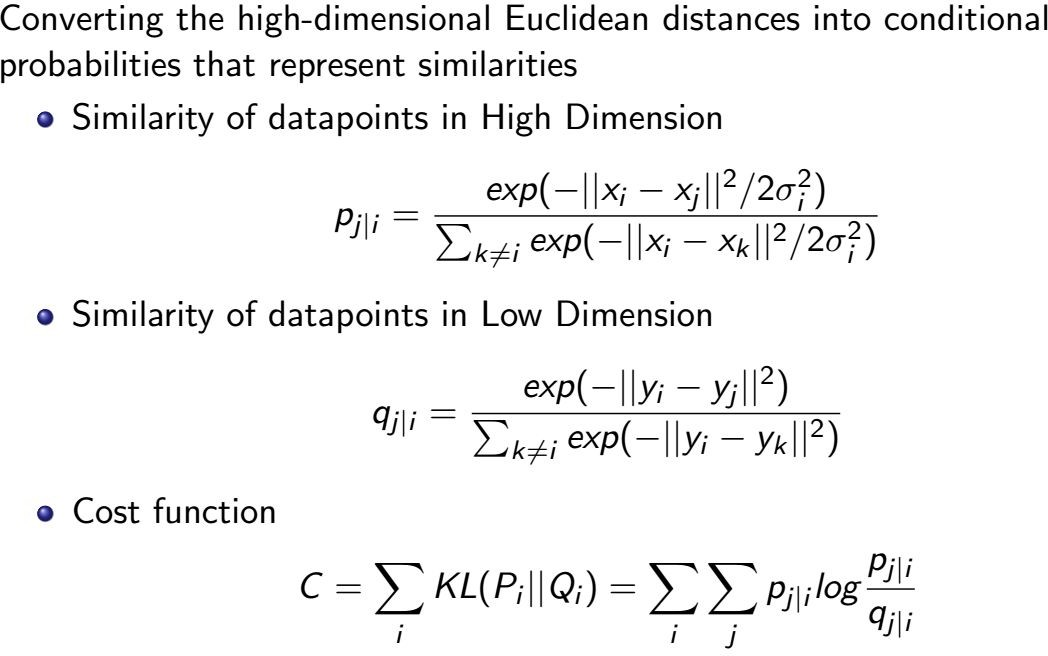
\includegraphics[width=1\textwidth,keepaspectratio]{images/dul/dim-reduce/tsne-stochastic-steps.jpg}
    \end{figure}
\end{frame}

\begin{frame}[allowframebreaks]{KL Divergence}
    \begin{columns}
    \begin{column}{0.4\textwidth}
        Measures the similarity between two probability distributions & it is asymmetric.

        \vspace{1em}

        \begin{figure}
            \centering
            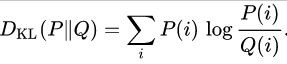
\includegraphics[width=1\textwidth,keepaspectratio]{images/dul/dim-reduce/tsne-similarity.jpg}
        \end{figure}
    \end{column}
    \begin{column}{0.6\textwidth}
        \begin{figure}
            \centering
            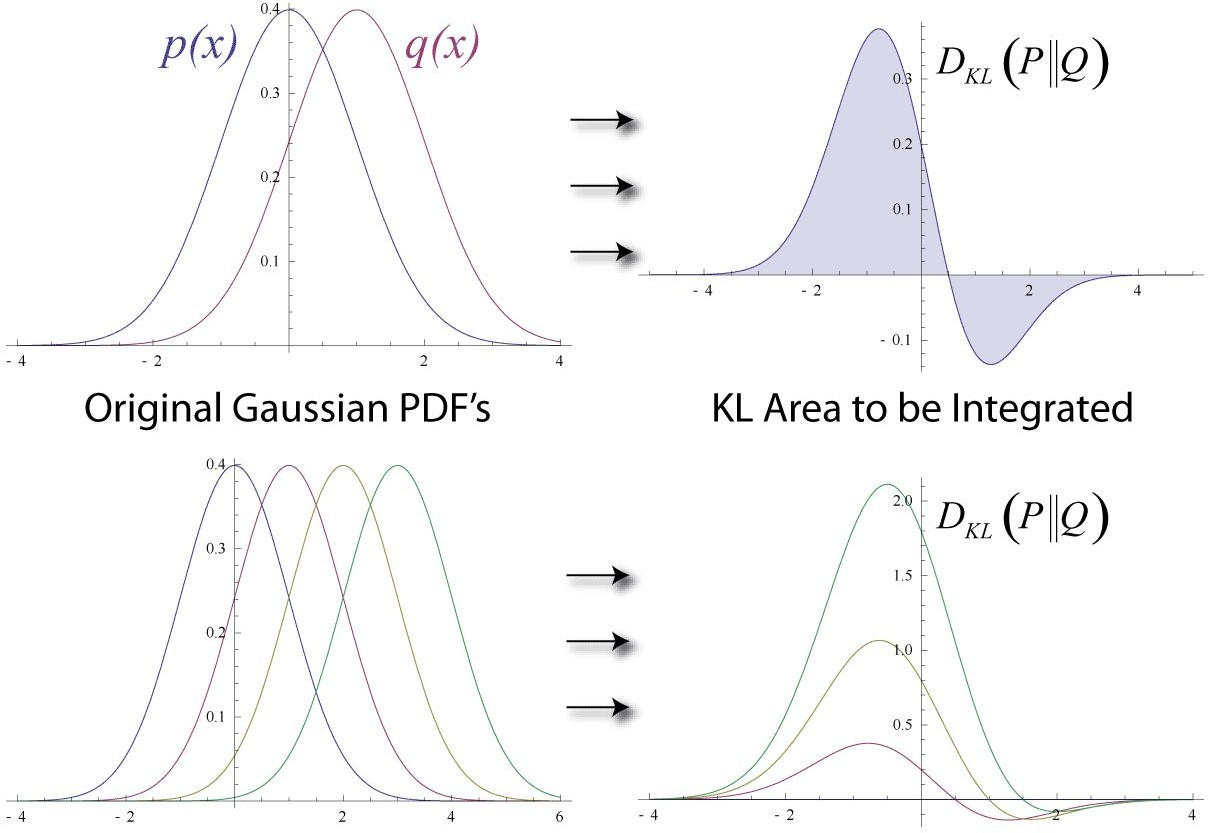
\includegraphics[width=1\textwidth,keepaspectratio]{images/dul/dim-reduce/tsne-similarity-graph.jpg}
        \end{figure}
    \end{column}
    \end{columns}
\end{frame}

\begin{frame}[allowframebreaks]{tSNE: Stochastic Neighbor Embedding}
    \begin{figure}
        \centering
        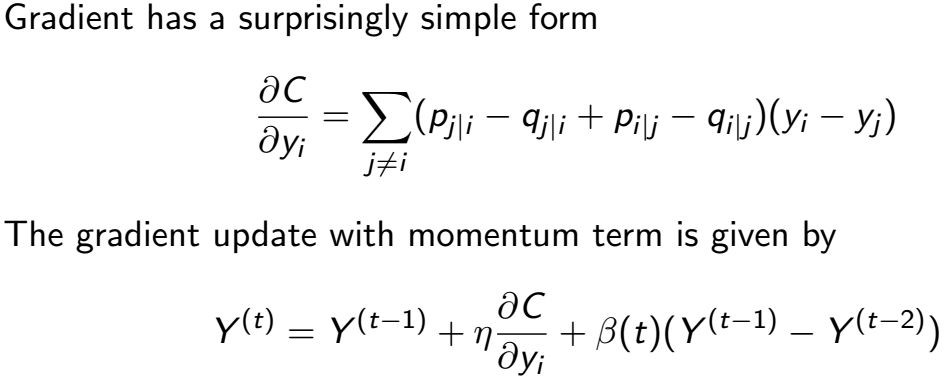
\includegraphics[width=1\textwidth,keepaspectratio]{images/dul/dim-reduce/tsne-gradient.jpg}
    \end{figure}

    \framebreak

    \begin{columns}
    \begin{column}{0.4\textwidth}
        \begin{itemize}
            \item The result of running the SNE algorithm on 3000 256-dimensional grayscale images of handwritten digits.
            \item The classes are quite well separated even though SNE had no information about class labels.
            \item Furthermore, within each class, properties like orientation, skew, and stroke thickness tend to vary smoothly across the space.
        \end{itemize}
    \end{column}
    \begin{column}{0.6\textwidth}
        \begin{figure}
            \centering
            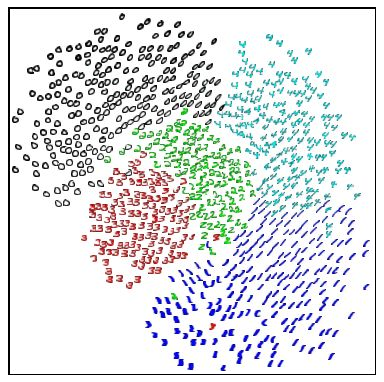
\includegraphics[width=1\textwidth,keepaspectratio]{images/dul/dim-reduce/tsne-result-1.png}
        \end{figure}
    \end{column}
    \end{columns}
\end{frame}

\begin{frame}[allowframebreaks]{Symmetric SNE}
    \begin{figure}
        \centering
        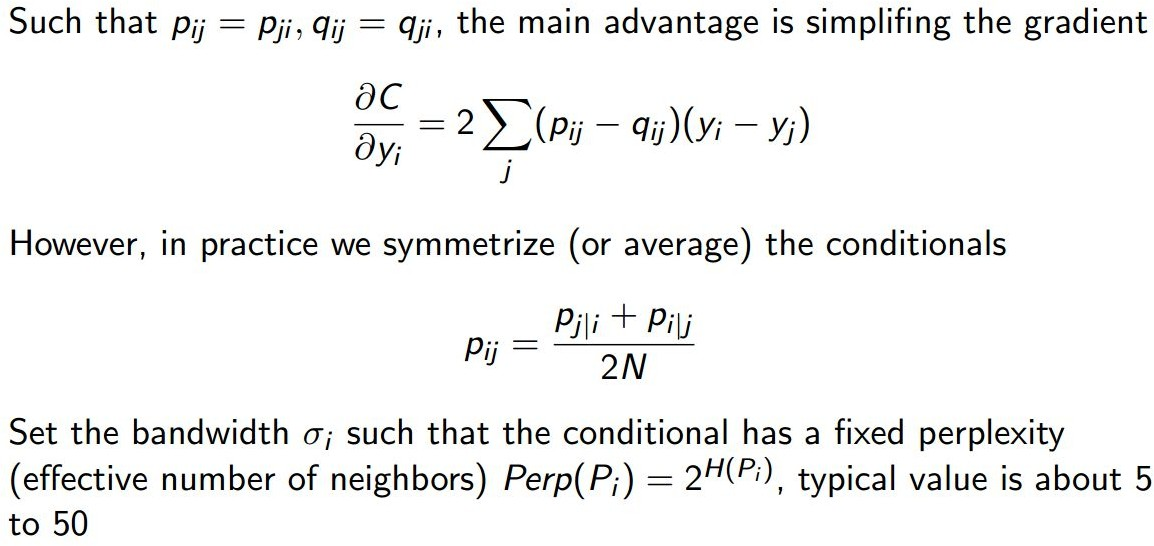
\includegraphics[width=1\textwidth,keepaspectratio]{images/dul/dim-reduce/symmetric-sne.jpg}
    \end{figure}
\end{frame}

\begin{frame}[allowframebreaks]{t-Distribution}
    \begin{figure}
        \centering
        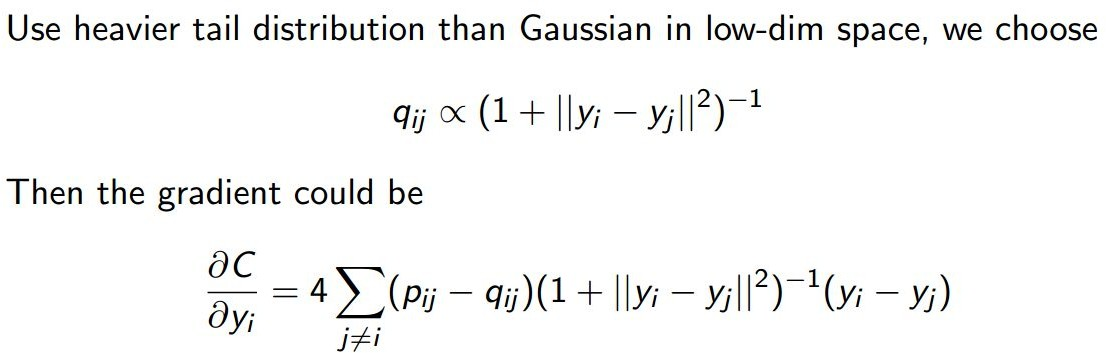
\includegraphics[width=1\textwidth,keepaspectratio]{images/dul/dim-reduce/t-distribution.jpg}
    \end{figure}
\end{frame}

\begin{frame}[allowframebreaks]{Student's t-Distribution}
    \begin{columns}
    \begin{column}{0.5\textwidth}
        \begin{itemize}
            \item Why do we define map similarities as:
            \begin{equation*}
                q_{ij} = \frac{(1 + \|y_i - y_j\|^2)^{-1}}{\sum_{k \neq l} (1 + \|y_k - y_l\|^2)^{-1}}
            \end{equation*}
            \item Suppose data is intrinsically high dimensional
            \item We try to model the local structure of this data in the map
            \item Result: Dissimilar points have to be modeled as too far apart in the map!
        \end{itemize}
    \end{column}
    \begin{column}{0.5\textwidth}
        \begin{figure}
            \centering
            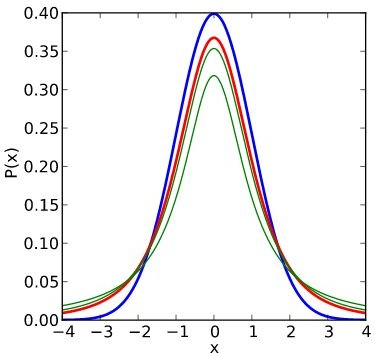
\includegraphics[width=1\textwidth,keepaspectratio]{images/dul/dim-reduce/stundets-t-distrubution.jpg}
        \end{figure}
    \end{column}
    \end{columns}
\end{frame}

\begin{frame}[allowframebreaks]{t-Distributed Stochastic Neighbor Embedding}
    \begin{figure}
        \centering
        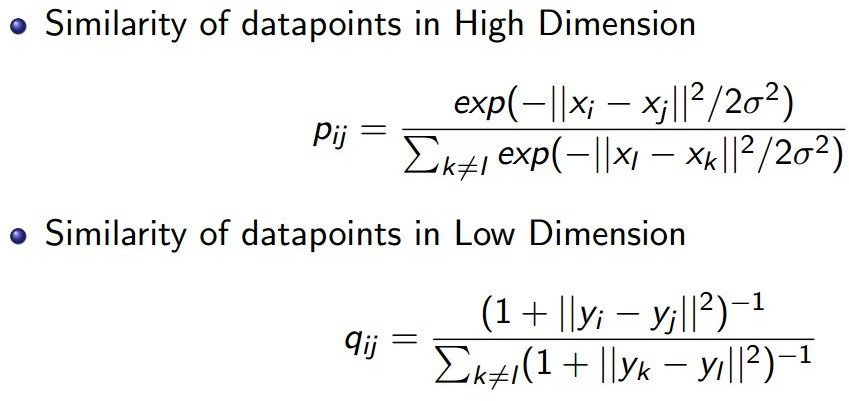
\includegraphics[width=1\textwidth,keepaspectratio]{images/dul/dim-reduce/t-distributed-stochastic.jpg}
    \end{figure}

    \framebreak

    \begin{figure}
        \centering
        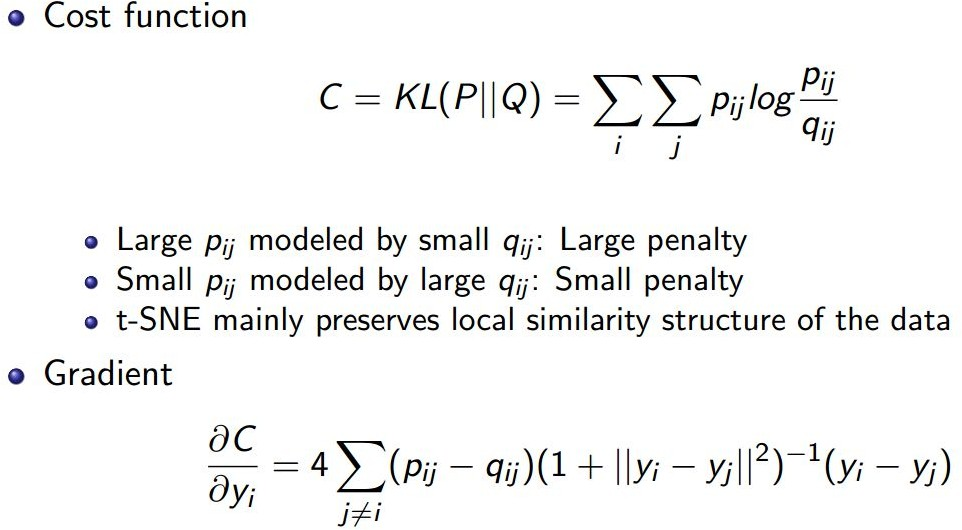
\includegraphics[width=1\textwidth,keepaspectratio]{images/dul/dim-reduce/t-distributed-stochastic-cost.jpg}
    \end{figure}
\end{frame}

\begin{frame}[allowframebreaks]{Distance scaling and perplexity}
    \begin{itemize}
        \item Perplexity = expected number of neighbours within a cluster
        \item Distances scaled relative to perplexity neighbours
    \end{itemize}
    \begin{columns}
    \begin{column}{0.5\textwidth}
        \begin{figure}
            \centering
            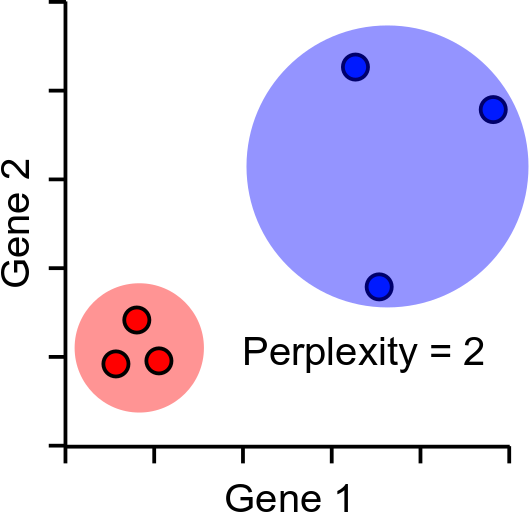
\includegraphics[width=1\textwidth,keepaspectratio]{images/dul/dim-reduce/tsne-distance-scaling.png}
        \end{figure}
    \end{column}
    \begin{column}{0.5\textwidth}
        \begin{figure}
            \centering
            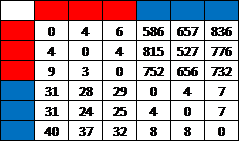
\includegraphics[width=1\textwidth,keepaspectratio]{images/dul/dim-reduce/tsne-distance-scaling-matrix.png}
        \end{figure}
    \end{column}
    \end{columns}
\end{frame}

\begin{frame}[allowframebreaks]{Perplexity Robustness}
    \begin{columns}
    \begin{column}{0.33\textwidth}
        \begin{figure}
            \centering
            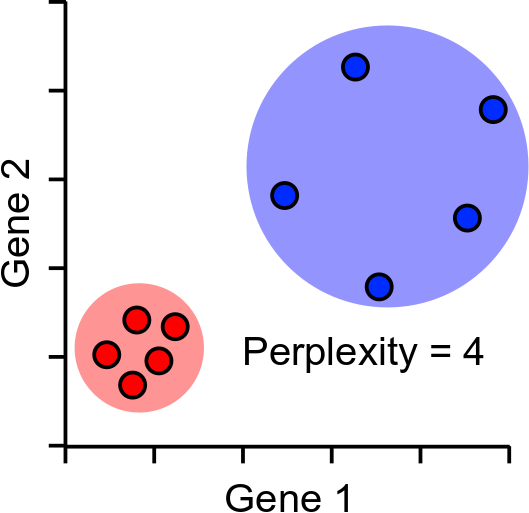
\includegraphics[width=1\textwidth,keepaspectratio]{images/dul/dim-reduce/slide_29_1_img.png}
        \end{figure}
    \end{column}
    \begin{column}{0.33\textwidth}
        \begin{figure}
            \centering
            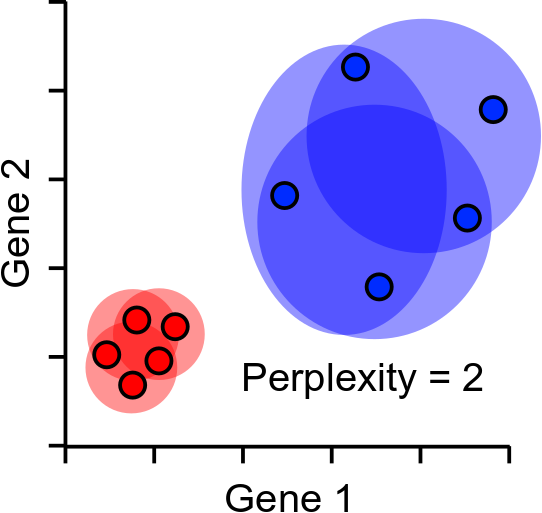
\includegraphics[width=1\textwidth,keepaspectratio]{images/dul/dim-reduce/slide_29_2_img.png}
        \end{figure}
    \end{column}
    \begin{column}{0.33\textwidth}
        \begin{figure}
            \centering
            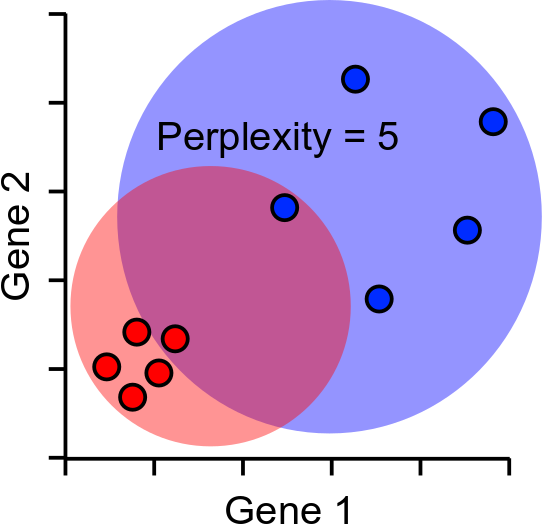
\includegraphics[width=1\textwidth,keepaspectratio]{images/dul/dim-reduce/slide_29_3_img.png}
        \end{figure}
    \end{column}
    \end{columns}
\end{frame}

\begin{frame}[allowframebreaks]{tSNE Projection}
    \begin{itemize}
        \item Randomly scatter all points within the space (normally 2D)
        \item Start a simulation
        \begin{itemize}
            \item Aim is to make the point distances match the distance matrix
            \item Shuffle points based on how well they match
            \item Stop after fixed number of iterations, or
            \item Stop after distances have converged
        \end{itemize}
    \end{itemize}

    \framebreak

    \begin{columns}
    \begin{column}{0.2\textwidth}
        \begin{figure}
            \centering
            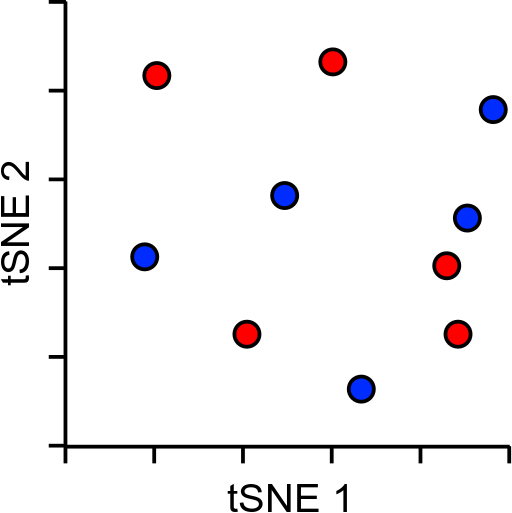
\includegraphics[width=1\textwidth,keepaspectratio]{images/dul/dim-reduce/slide_31_1_img.png}
        \end{figure}
    \end{column}
    \begin{column}{0.2\textwidth}
        \begin{figure}
            \centering
            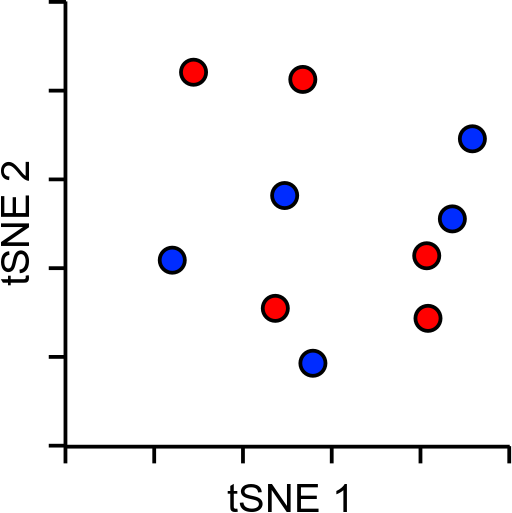
\includegraphics[width=1\textwidth,keepaspectratio]{images/dul/dim-reduce/slide_31_2_img.png}
        \end{figure}
    \end{column}
    \begin{column}{0.2\textwidth}
        \begin{figure}
            \centering
            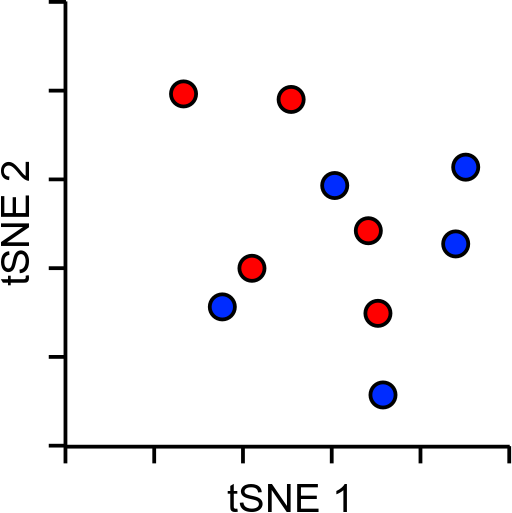
\includegraphics[width=1\textwidth,keepaspectratio]{images/dul/dim-reduce/slide_31_3_img.png}
        \end{figure}
    \end{column}
    \begin{column}{0.2\textwidth}
        \begin{figure}
            \centering
            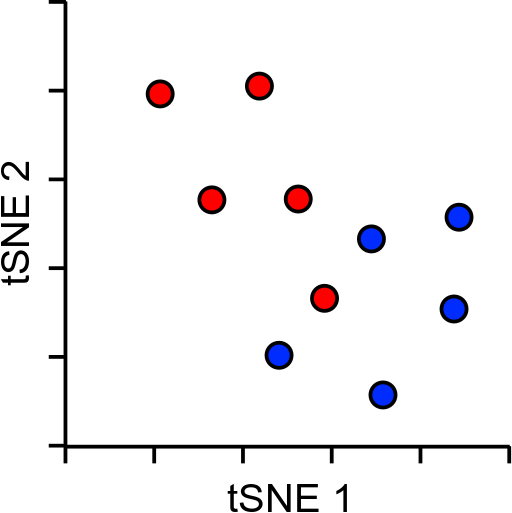
\includegraphics[width=1\textwidth,keepaspectratio]{images/dul/dim-reduce/slide_31_4_img.png}
        \end{figure}
    \end{column}
    \begin{column}{0.2\textwidth}
        \begin{figure}
            \centering
            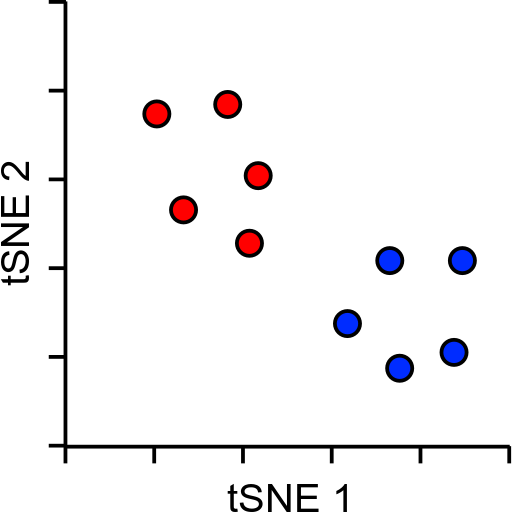
\includegraphics[width=1\textwidth,keepaspectratio]{images/dul/dim-reduce/slide_31_5_img.png}
        \end{figure}
    \end{column}
    \end{columns}

    \vspace{3em}
    \begin{itemize}
        \item X and Y don’t mean anything (unlike PCA)
        \item Distance doesn’t mean anything (unlike PCA)
        \item Close proximity is highly informative
        \item Distant proximity isn’t very interesting
        \item Can’t rationalise distances, or add in more data
    \end{itemize}
\end{frame}

\begin{frame}[allowframebreaks]{tSNE: Practical Examples}
    \begin{figure}
        \centering
        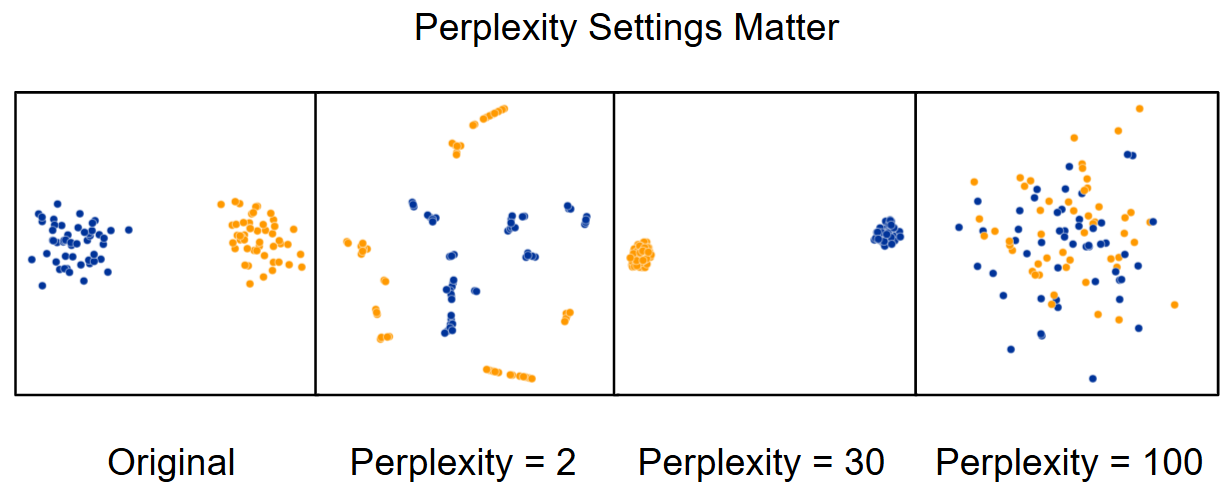
\includegraphics[width=1\textwidth,keepaspectratio]{images/dul/dim-reduce/tsne-perplexity-settings.png}
    \end{figure}

    \framebreak

    \begin{figure}
        \centering
        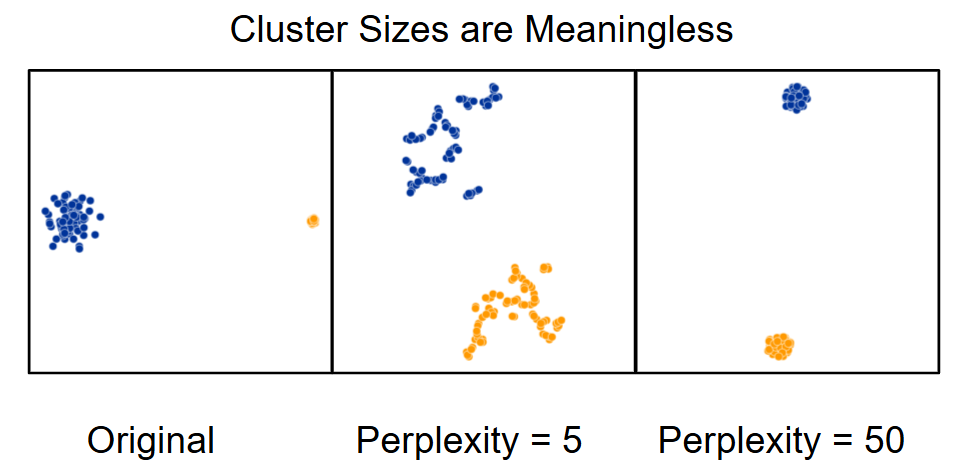
\includegraphics[width=1\textwidth,keepaspectratio]{images/dul/dim-reduce/tsne-perplexity-settings-2.png}
    \end{figure}

    \framebreak

    \begin{figure}
        \centering
        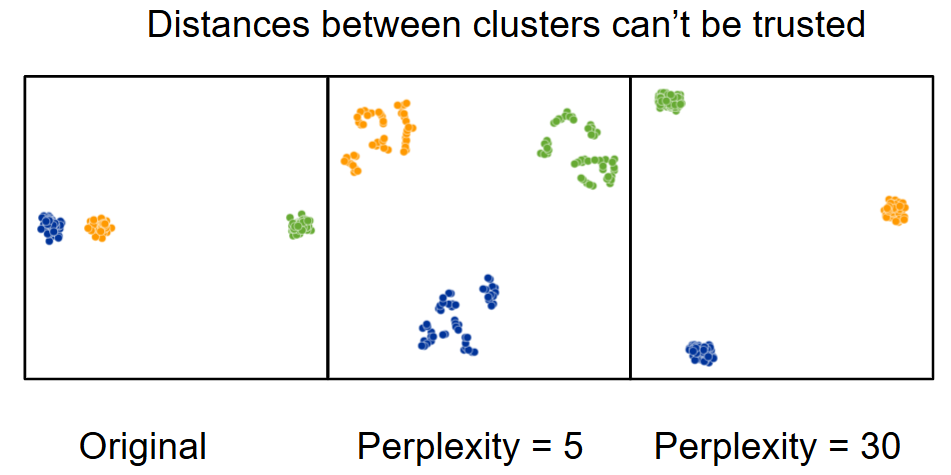
\includegraphics[width=1\textwidth,keepaspectratio]{images/dul/dim-reduce/tsne-perplexity-settings-3.png}
    \end{figure}
\end{frame}

\begin{frame}[allowframebreaks]{tSNE: Results on MNIST}
    \begin{figure}
        \centering
        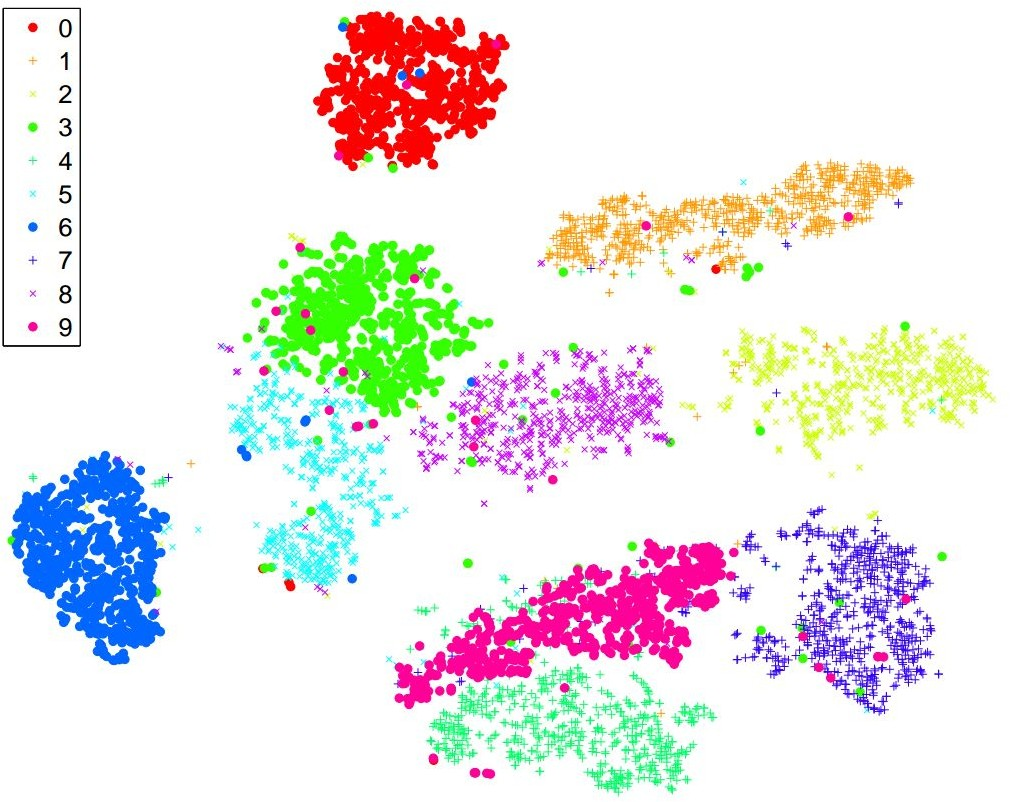
\includegraphics[width=0.9\textwidth,keepaspectratio]{images/dul/dim-reduce/slide_35_1_img.jpg}
    \end{figure}
\end{frame}

\begin{frame}[allowframebreaks]{So tSNE is great then?}
    Kind of\dots

    Imagine a dataset with only one super informative gene

    \begin{columns}
    \begin{column}{0.33\textwidth}
        \begin{figure}
            \centering
            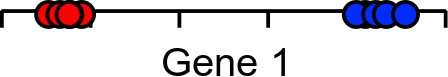
\includegraphics[width=1\textwidth,keepaspectratio]{images/dul/dim-reduce/slide_36_1_img.png}
        \end{figure}

        \vspace{1em}

Distance within cluster = low

\vspace{1em}
        
Distance between clusters = high
    \end{column}
    \begin{column}{0.33\textwidth}
        \begin{figure}
            \centering
            \includegraphics[width=1\textwidth,keepaspectratio]{images/dul/dim-reduce/slide_36_2_img.png}
        \end{figure}
        
        \vspace{1em}

Distance within cluster = higher

\vspace{1em}
        
Distance between clusters = lower
    \end{column}
    \begin{column}{0.33\textwidth}
        \begin{itemize}
            \item First - 3 genes
            \item Second -  3,000 genes
            \item Everything is the same distance from everything
        \end{itemize}
    \end{column}
    \end{columns}
\end{frame}

\begin{frame}[allowframebreaks]{So there is no clear solution?}
    \begin{columns}
    \begin{column}{0.5\textwidth}
        PCA:
        \begin{itemize}
            \item Requires more than 2 dimensions
            \item Expects linear relationships
        \end{itemize}
    \end{column}
    \begin{column}{0.5\textwidth}
        tSNE:
        \begin{itemize}
            \item Can’t cope with noisy data
            \item Loses the ability to cluster
        \end{itemize}
    \end{column}
    \end{columns}

    \framebreak

    \begin{columns}
    \begin{column}{0.5\textwidth}
        PCA:
        \begin{itemize}
            \item Requires more than 2 dimensions
            \item Expects linear relationships
        \end{itemize}
    \end{column}
    \begin{column}{0.5\textwidth}
        tSNE:
        \begin{itemize}
            \item Can’t cope with noisy data
            \item Loses the ability to cluster
        \end{itemize}
    \end{column}
    \end{columns}
    \vspace{1em}
    \textbf{Answer: Combine the two methods, get the best of both worlds!}
    \vspace{1em}
    \begin{columns}
    \begin{column}{0.5\textwidth}
        PCA:
        \begin{itemize}
            \item Good at extracting signal from noise
            \item Extracts informative dimensions
        \end{itemize}
    \end{column}
    \begin{column}{0.5\textwidth}
        tSNE:
        \begin{itemize}
            \item Can reduce to 2D well
            \item Can cope with non-linear scaling
        \end{itemize}
    \end{column}
    \end{columns}
    \vspace{1em}
    \textbf{This is what many pipelines do in their default analysis!}

\end{frame}

\begin{frame}[allowframebreaks]{So PCA + tSNE is great then?}
    Kind of\dots
    \begin{itemize}
        \item tSNE is slow—this is its biggest drawback.
        \begin{itemize}
            \item tSNE does not scale well to large datasets (10,000+ samples).
        \end{itemize}
        \item tSNE provides reliable information only about the closest neighbors; large distance information is mostly irrelevant.
    \end{itemize}
\end{frame}
\begin{frame}[allowframebreaks]{UMAP to the rescue!}
    \begin{itemize}
        \item UMAP is a replacement for t-SNE, designed to fulfill the same role in dimensionality reduction.
        \item It is conceptually very similar to t-SNE, but introduces several relevant (and somewhat technical) changes.
        \item In practice, UMAP offers several advantages:
        \begin{itemize}
            \item UMAP is significantly faster than t-SNE.
            \item It can preserve more global structure compared to t-SNE.\footnote{Preservation of global structure may depend on the dataset and parameter choices.}
            \item UMAP can operate directly on raw data without requiring PCA preprocessing.\footnote{Although PCA preprocessing can still be beneficial in some cases.}
            \item It allows new data points to be added to an existing projection, enabling incremental updates.
        \end{itemize}
    \end{itemize}
\end{frame}


\begin{frame}[allowframebreaks]{UMAP differences}
    \begin{itemize}
        \item Unlike t-SNE, which uses a single perplexity parameter, UMAP introduces two key parameters:
        \begin{itemize}
            \item \textbf{Number of Nearest Neighbours:} Specifies how many nearest neighbours are considered for each point. This is conceptually similar to perplexity in t-SNE and controls the balance between local and global structure in the embedding.
            \item \textbf{Minimum Distance:} Determines how closely UMAP packs points together in the low-dimensional space. Lower values allow points to be closer, resulting in more compact clusters, while higher values spread points apart.
        \end{itemize}
        \item The \textbf{nearest neighbours} parameter influences the trade-off between preserving local versus global structure in the data.
        \item The \textbf{minimum distance} parameter affects the density and compactness of clusters in the resulting visualization.
        \item Together, these parameters provide more flexibility and control over the embedding compared to t-SNE's single perplexity value.
    \end{itemize}

    \framebreak

    \textbf{Structure preservation} – mostly in the 2D projection scoring
    \vspace{1em}
    \begin{columns}
    \begin{column}{0.4\textwidth}
        \begin{figure}
            \centering
            \includegraphics[width=1\textwidth,keepaspectratio]{images/dul/dim-reduce/slide_41_1_img.png}
            \caption{t-SNE}
        \end{figure}
    \end{column}
    \begin{column}{0.4\textwidth}
        \begin{figure}
            \centering
            \includegraphics[width=1\textwidth,keepaspectratio]{images/dul/dim-reduce/slide_41_2_img.png}
            \caption{UMAP}
        \end{figure}
    \end{column}
    \begin{column}{0.22\textwidth}
        \begin{figure}
            \centering
            \includegraphics[width=1\textwidth,keepaspectratio]{images/dul/dim-reduce/slide_41_3_img.png}
        \end{figure}
    \end{column}
    \end{columns}
\end{frame}

\begin{frame}[allowframebreaks]{So UMAP is great then?}
    \begin{figure}
        \centering
        \includegraphics[width=1\textwidth,keepaspectratio]{images/dul/dim-reduce/slide_42_1_img.png}
    \end{figure}
\end{frame}

\begin{frame}[allowframebreaks]{So UMAP is all hype then?}
    \begin{figure}
        \centering
        \includegraphics[width=1\textwidth,keepaspectratio]{images/dul/dim-reduce/slide_43_1_img.png}
    \end{figure}
\end{frame}


\begin{frame}[allowframebreaks]{Practical approach PCA + tSNE/UMAP}
    \begin{itemize}
        \item \textbf{Filter the data:}
        \begin{itemize}
            \item Remove poorly behaving cells to ensure data quality.
            \item Select only expressed genes for further analysis.
            \item Identify and retain variable genes to focus on informative features.
        \end{itemize}
        \item \textbf{Apply PCA (Principal Component Analysis):}
        \begin{itemize}
            \item Extract the most interesting and informative signals from the data.
            \item Select the top principal components (PCs) to reduce dimensionality, but do not reduce directly to 2 dimensions.
        \end{itemize}
        \item \textbf{Run t-SNE or UMAP:}
        \begin{itemize}
            \item Calculate distances between samples using the PCA projections.
            \item Scale these distances appropriately.
            \item Project the data into 2 dimensions for visualization using t-SNE or UMAP.
        \end{itemize}
    \end{itemize}
\end{frame}

\begin{frame}[allowframebreaks]{So PCA + UMAP is great then?}
    \begin{columns}
    \begin{column}{0.4\textwidth}
        \begin{itemize}
            \item Kind of\ldots{} as long as you only have one dataset.
            \begin{itemize}
                \item In 10X experiments, each library is considered a \textbf{batch}.
                \item Over time or distance, additional biases can be introduced.
                \item These biases make direct comparisons between datasets challenging.
                \item To enable meaningful comparisons, it is necessary to align the datasets and correct for batch effects.
            \end{itemize}
        \end{itemize}
    \end{column}
    \begin{column}{0.6\textwidth}
        \begin{figure}
            \centering
            \includegraphics[width=1\textwidth,keepaspectratio]{images/dul/dim-reduce/slide_45_1_img.png}
            \caption{UMAP}
        \end{figure}
    \end{column}
    \end{columns}
\end{frame}